\documentclass{article}

\usepackage[letterpaper]{geometry}
\usepackage{amsmath}
\usepackage{graphicx}

\graphicspath{{./img/}}

\title{2411 HW 7}
\author{Duncan Wilkie}
\date{25 October 2021}

\begin{document}
\section{}
The corresponding program appears in the script files section.

\section{}
Gaussian elimination may be applied to solve the matrix inverse problem $\mathbf{A}\vec{x}=\vec{b}$. All linear systems of equations, where one has some linear combination of variables equal to a constant in each of the eqations, may be written as a problem of this form. Classify the use of Gaussian elimination to find that a system is over- or underdetermined as ``solving'' the system of equations (otherwise, one would need to actualy solve the system to determine if a well-defined solution were possible).
\subsection{}
This one can be reduced to a linear system by setting $x = \cos(\alpha)$ and $y = \tan^2(\phi)$. Gaussian elimination becomes directly applicable.
\subsection{}
Expanding $(u-2v)^2=u^2-4uv+4v^2$, it becomes evident we may linearize the system by setting $x = u^2$, $y=v^2$. Gaussian elimination becomes directly applicable.
\subsection{}
This requires pivoting, since the first row contains a zero as its first entry. 
\subsection{}
Once again, Gaussian elimination is directly applicable.
\subsection{}
In this case, it is impossible to write $e^z$ as a linear function of $z$ (stated without proof---technically follows from a polynomial-ring-over-field proof of it being a trancendental function, which is highly nontrivial). Therefore, this cannot be reduced to a linear system, and Gaussian elimination is impossible to apply.

\section{}
The first print statement outputs
\[\begin{bmatrix}
    1 & 8 & 10\\
    2 & 1 & 11\\
    5 & -50 & -14
  \end{bmatrix}\]
The second print statement outputs the superposed version of the matrix from the in-place decomposition algorithm (the ``Hadamard sum,'' I suppose):
\[\begin{bmatrix}
    1 & 8 & 10 \\
    2 & -15 & -9 \\
    5 & 6 & -10
  \end{bmatrix}\]
\section{}
The program modified for this problem appears in the script files. The plot of $\log f(x)$ appears below for both roots.
\[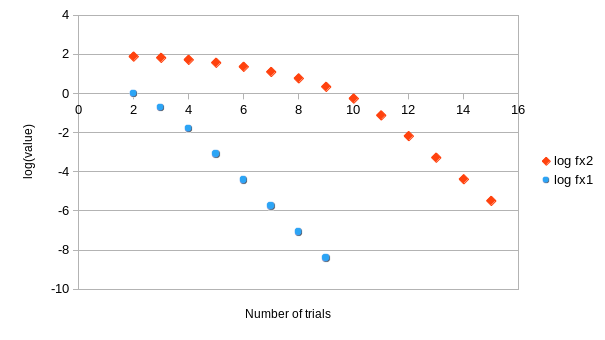
\includegraphics[scale=0.5]{plot1.png}\]
It is evident that the dependence obeys a negative power law for the first root, and approaches a negative power law for the second root. There is better convergence in the analytical case compared to this one. 
\section*{Script Files}
\subsection*{1}
\begin{verbatim}
Script started, file is dwilk14_hw7p1.txt
[dwilk14@tigers ~/HW7]$ cat dwilk14_hw7p1.cpp
#include <fstream>

using namespace std;

int main() {
  ofstream outfile;
  outfile.open("output.txt");
  float A[5][5];

  for (int i = 0; i < 5; i++) {
    for (int j = 0; j < 5; j++) {
      A[i][j] = (j >= i) ? -i + j + 1: 0;
    }
  }

  float b[5] = {3, 2.03, 1.16, 0.44, 0.02};

  float x[5];
  for (int i = 4; i >=0; i--) {
    x[i] = b[i];
    for (int j = i + 1; j < 5; j++) {
      x[i] -= A[i][j] * x[j];
    }
  }

  for (int i = 0; i < 5; i++) {
    outfile << x[i] << " ";
  }

  outfile << endl;

  return 0;

}
[dwilk14@tigers ~/HW7]$ g++ dwilk14_hw7p1.cpp -o dwilk14_hw7p1
[dwilk14@tigers ~/HW7]$ ./dwilk14_hw7p1
[dwilk14@tigers ~/HW7]$ cp dwilk14_hw7p1.txt /home3/kristina/phys2411/.
[dwilk14@tigers ~/HW7]$ exit
exit
Script done, file is dwilk14_hw7p1.txt
\end{verbatim}

\subsection*{2}
\begin{verbatim}
Script started, file is dwilk14_hw7p2.txt
[dwilk14@tigers ~/HW7]$ cat dwilk14_hw7p2.cpp
#include <fstream>
#include <iostream>
#include <cmath>

using namespace std;

double f(double x) {
    return tan(x) - x;
}

double deriv(double x) {
  double h = 0.01;
  return (f(x + h) - f(x)) / h;
}

int main() {
  ofstream outfile;
  outfile.open("output2.txt");
  outfile.precision(10);
  double guess1 = 4.4,  guess2 = 7.6, fx1 = f(guess1), fx2 = f(guess2);


  outfile << "n, x1, fx1" << endl;

  for (int i = 0; i < 15; i++) {
    outfile << i << ", " << guess1 << ", " << fx1 << endl;

    if (abs(fx1) < 1e-8) {
      break;
    }

    guess1 -= fx1 / deriv(guess1);
    fx1 = f(guess1);

  }

  outfile << "n, x2, fx2" << endl;


  for (int i = 0; i < 15; i++) {
    outfile << i << ", " << guess2 << ", " << fx2 << endl;

    if (abs(fx2) < 1e-8) {
      break;
    }

    guess2 -= fx2 / deriv(guess2);
    fx2 = f(guess2);

  }

  return 0;

}
[dwilk14@tigers ~/HW7]$ g++ dwilk14_hw7p2.cpp -o dwilk14_hw7p2
[dwilk14@tigers ~/HW7]$ ./dwilk14_hw7p2
[dwilk14@tigers ~/HW7]$ cp dwilk14_hw7p2.txt /home3/kristina/phys2411/.
[dwilk14@tigers ~/HW7]$ exit
exit
Script done, file is dwilk14_hw7p2.txt
\end{verbatim}
\end{document}
%%% Local Variables:
%%% mode: latex
%%% TeX-master: t
%%% End:
